\section{System Perspective}

%A description and illustration of the:

\subsection{System Architecture}
%Design and architecture of your ITU-MiniTwit systems
%Important interactions of subsystems
The following sections will go through various viewpoints to describe the architecture of our system. All views are created in accordance with the UML approach from Christensen et al. \cite{christensen2016_uml}. 

\subsubsection{Module Viewpoint}

Figure \ref{fig:repo-visualized} shows a code visualization of our repository. In this view, generated by Amelia Wattenberger's codebase visualizer \cite{codebase_visualizer}, grey circles represent directories, while filled-in circles represent files, the color corresponding to a file format and its size to the file size. We include this view to give a broad overview of our repository and to give an idea of the size of the different files and directories, which is not possible to show with a package overview diagram. In addition, we point to the fact that the grafana, filebeat, and terraform directories lie outside the main application directory. Note that the \texttt{flag\_tool} directory and several \texttt{.md} files have been omitted from this view. \\

\begin{figure}[]
    \centering
    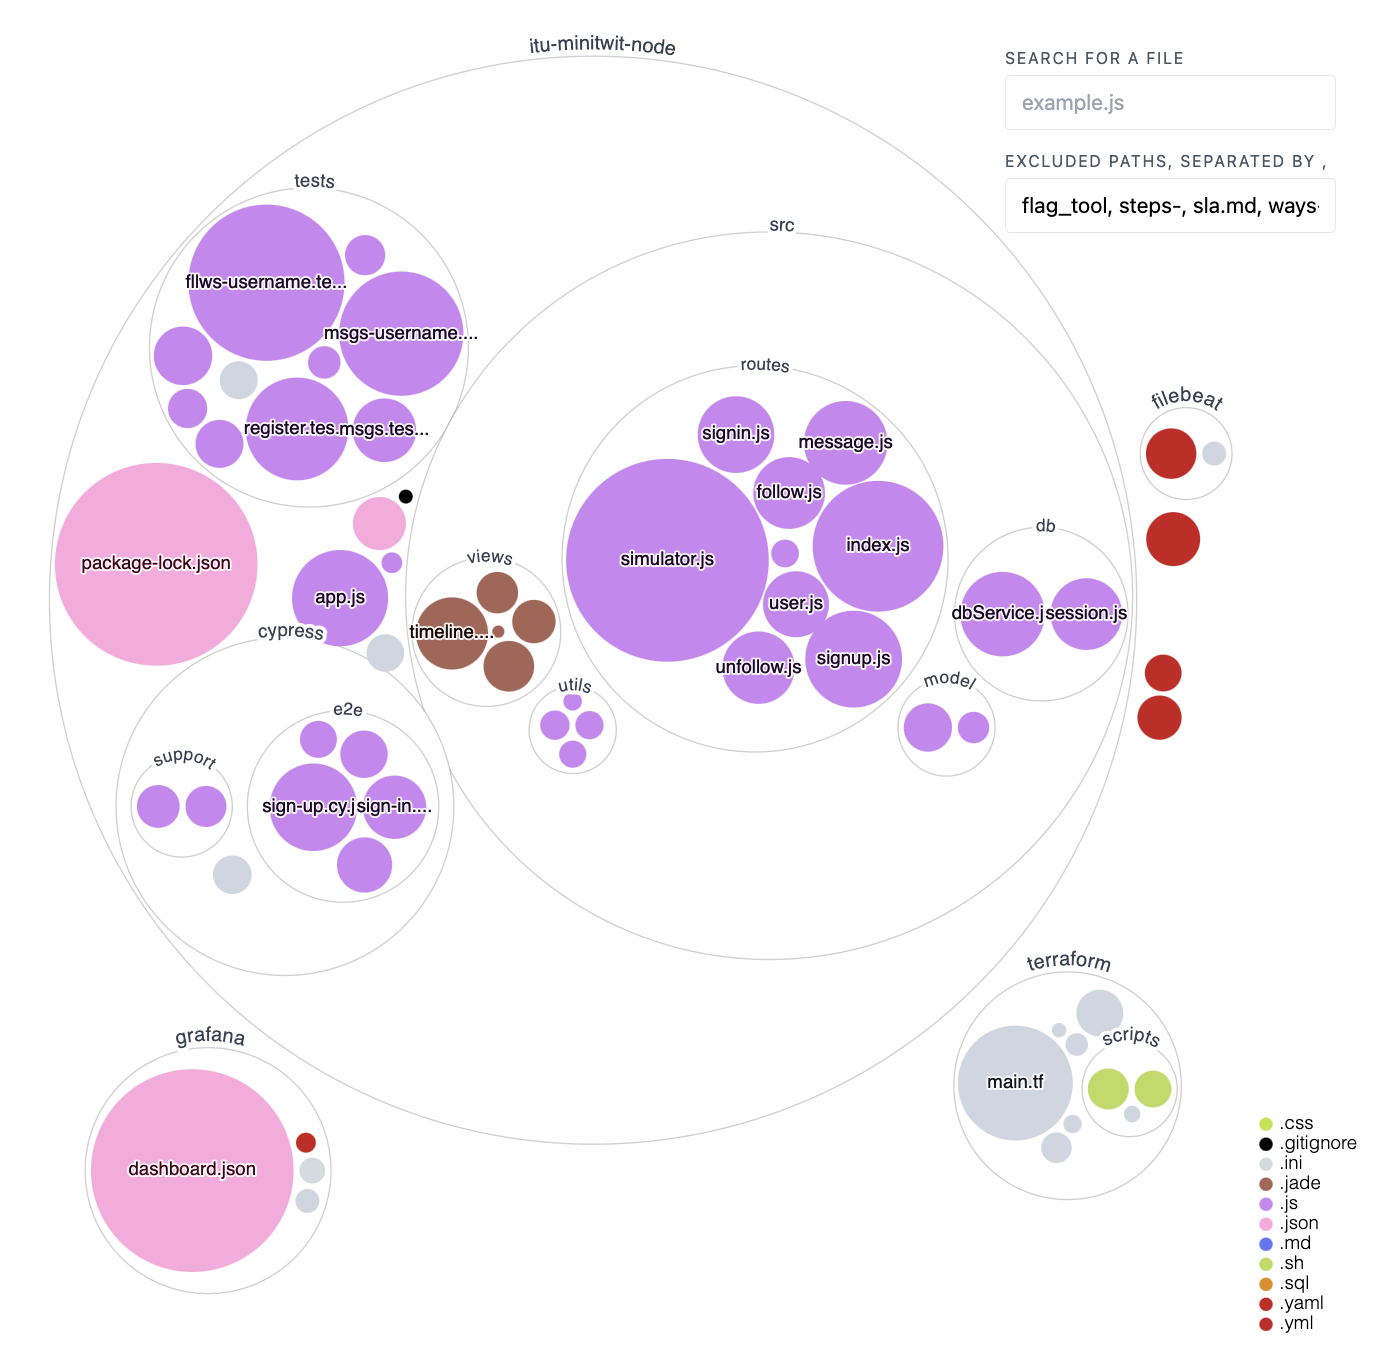
\includegraphics[width=\linewidth]{images/repo-visualizer.png}
    \caption{Visualization of our GitHub repository}
    \label{fig:repo-visualized}
\end{figure}

Figure \ref{fig:module-minitwit} shows a package overview diagram of the web app. Here we observe the dependencies between source files, the test directories, and the main \texttt{app.js} file. If we examine the \texttt{src} directory in more detail, as illustrated in Figure \ref{fig:module-src}, it becomes apparent that the \texttt{routes} directory relies heavily on various other components of the code, as all the app's endpoints are located within this directory. \\

\begin{figure}[H]
    \centering
    \begin{minipage}{0.45\textwidth}
        \centering
        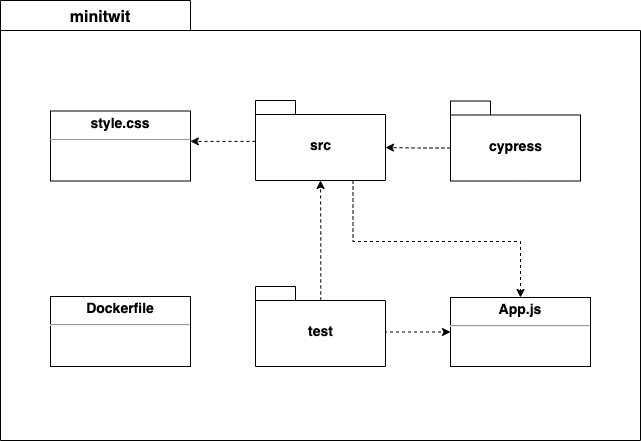
\includegraphics[width=.95\linewidth]{images/module-minitwit.png}
        \caption{Package overview diagram for the \texttt{minitwit} directory}
        \label{fig:module-minitwit}
    \end{minipage}\hfill
    \begin{minipage}{0.45\textwidth}
        \centering
        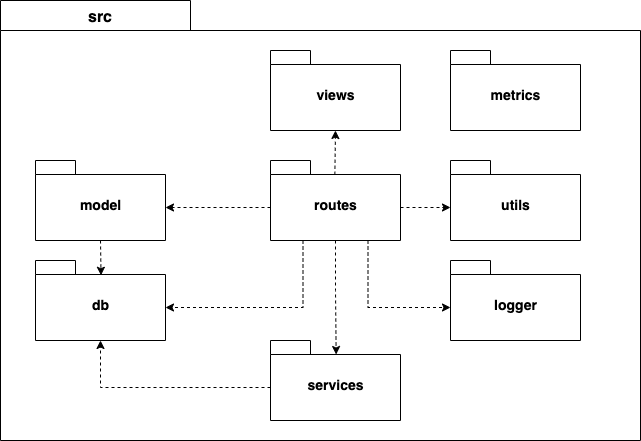
\includegraphics[width=.95\linewidth]{images/module-src.png}
        \caption{Decomposition of the \texttt{src} package}
        \label{fig:module-src}
    \end{minipage}
\end{figure}

\subsubsection{Component and Connector Viewpoint}

The sequence diagram shown in Figure \ref{fig:sequence-login} shows the interaction between subsystems in the scenario where a user successfully logs into the system. Had the username or password been wrong, the error would have been logged instead. \\

\begin{figure}[]
    \centering
    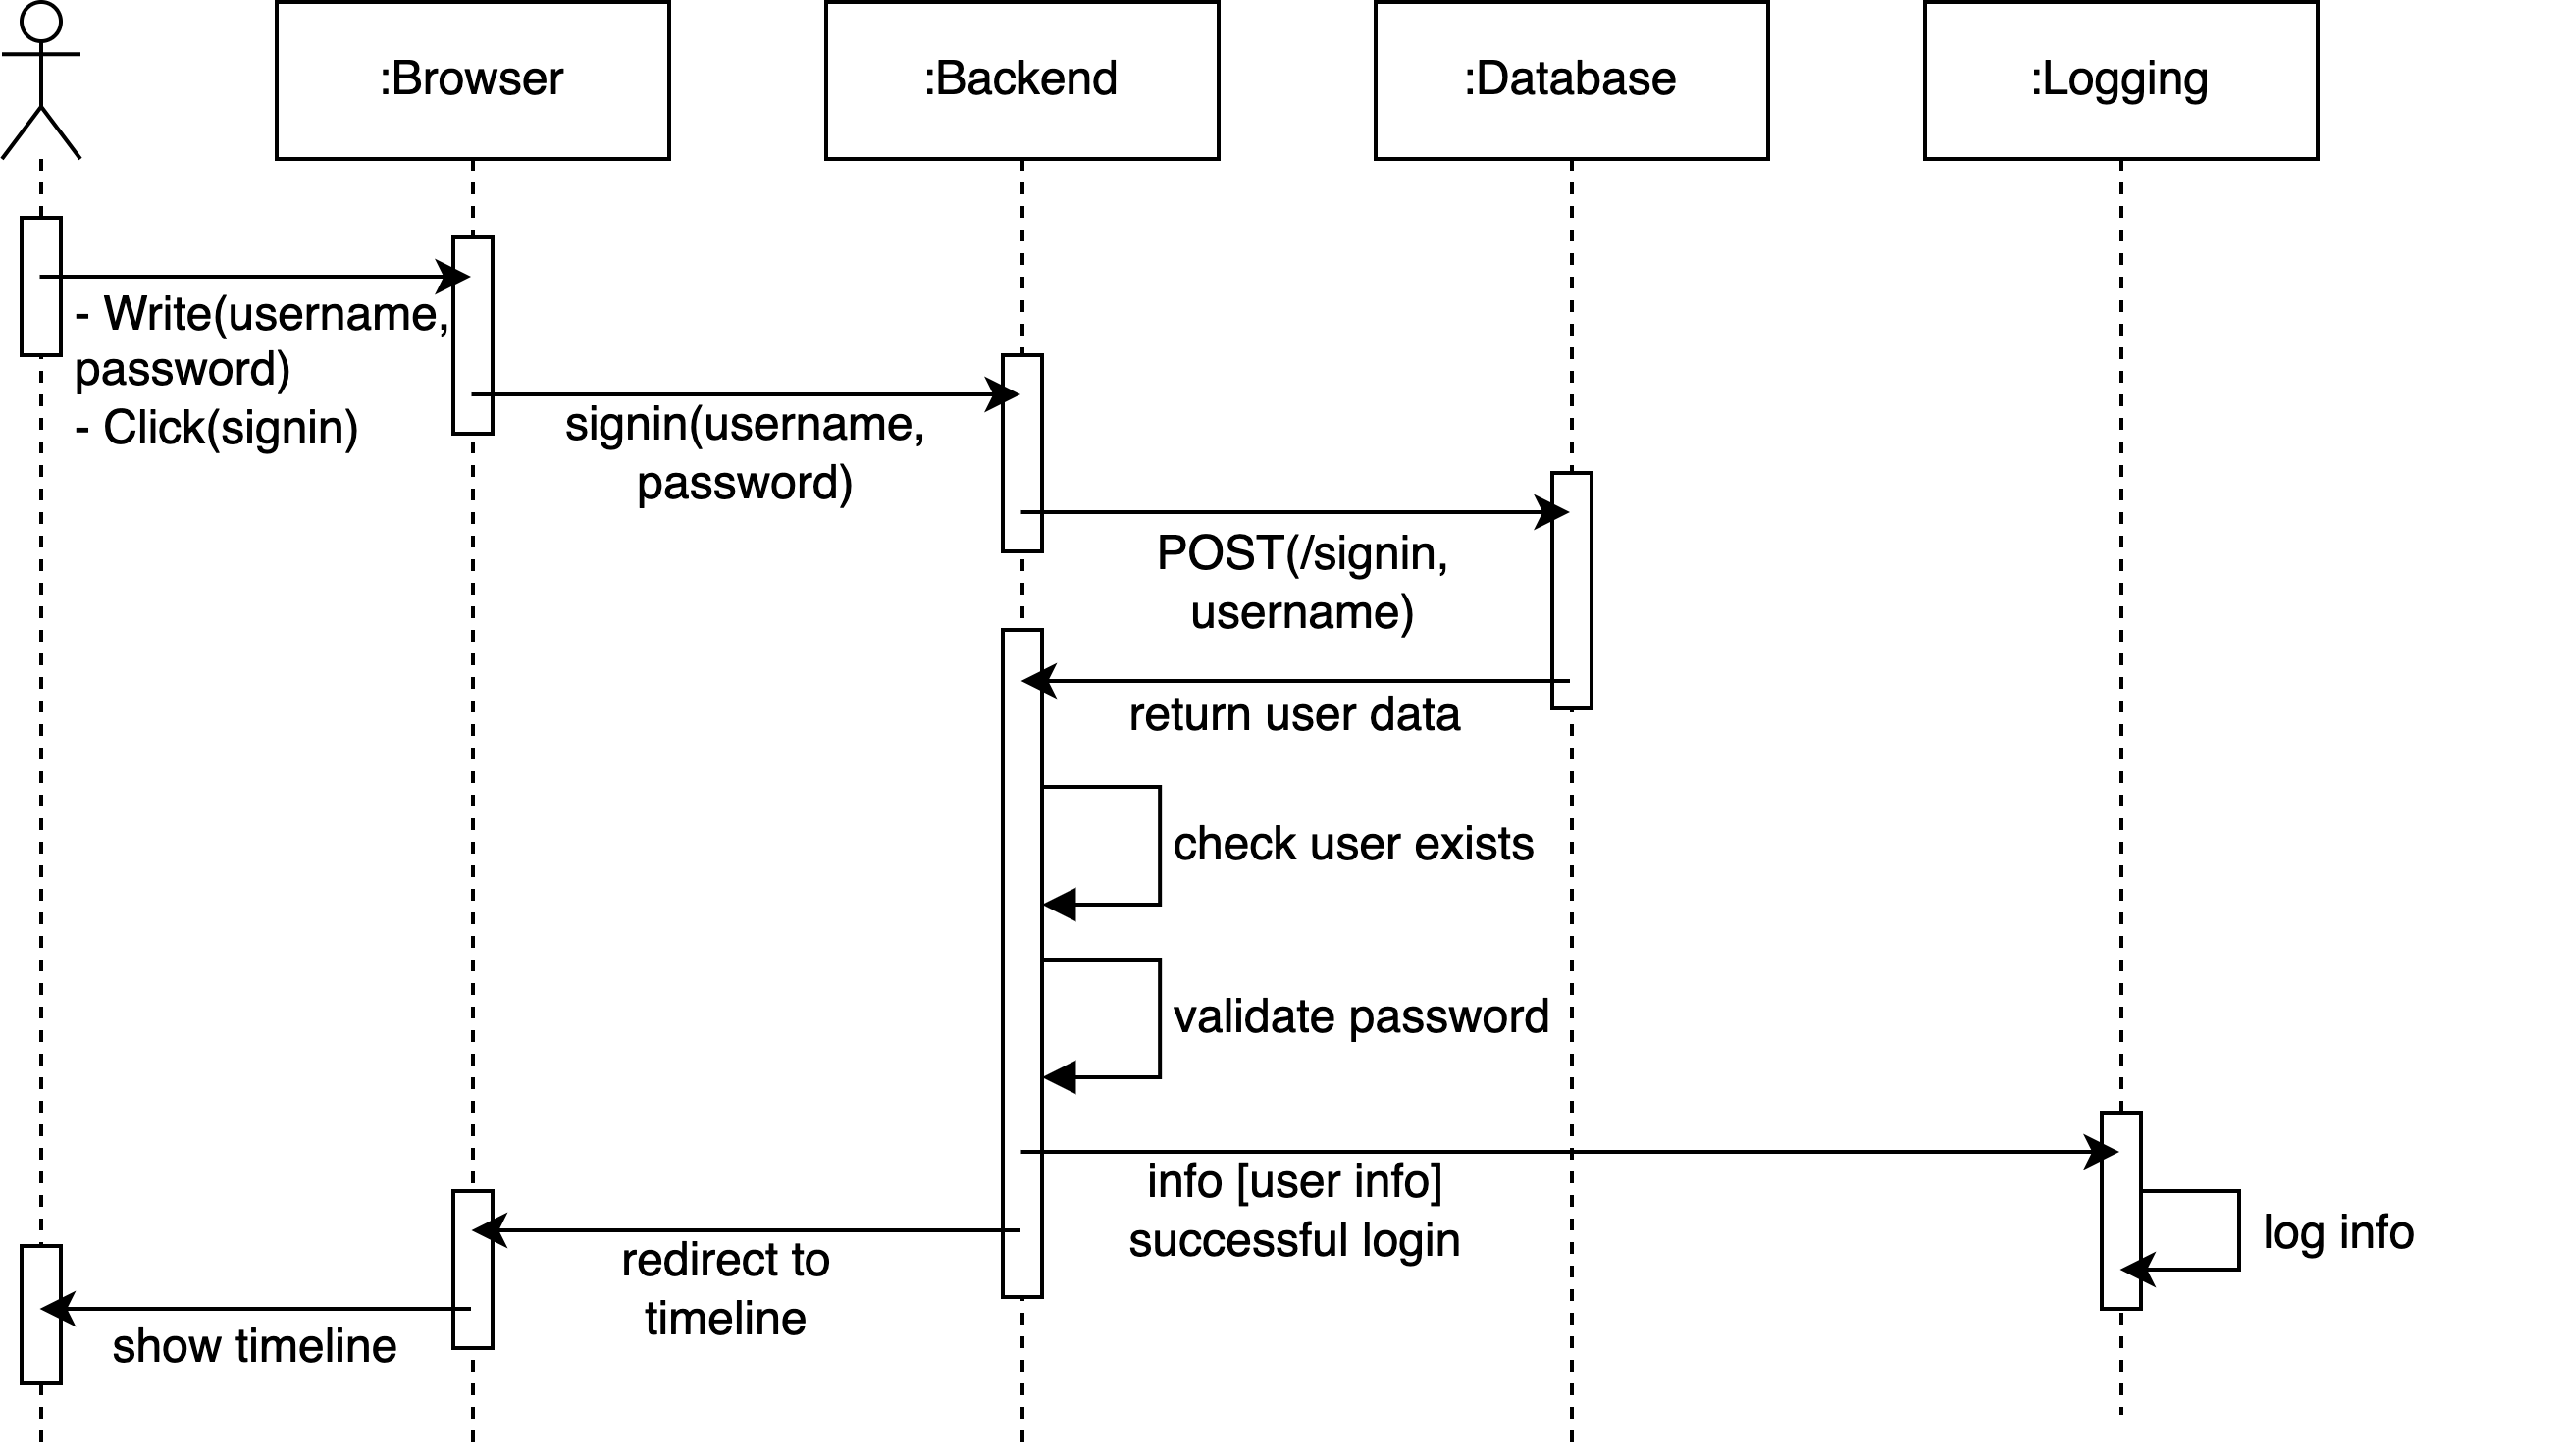
\includegraphics[width=\linewidth]{images/sequence-diagram.png}
    \caption{Sequence diagram of a successful login scenario}
    \label{fig:sequence-login}
\end{figure}

\subsubsection{Allocation Viewpoint}

Figure \ref{fig:deployment-diagram} shows a deployment view of our system. Note that dependencies among software elements have been omitted from this view. This view shows how our software elements are allocated to (virtual) environmental elements at runtime. Software elements in blue can be allocated to any of the environmental elements in red, in accordance with constraints put on our Docker Swarm. The elements in blue are in several layers (ex. the Minitwit component) if specified to be in several replicas.  

% Note that software elements marked in blue can be allocated to 

\begin{figure}[]
    \centering
    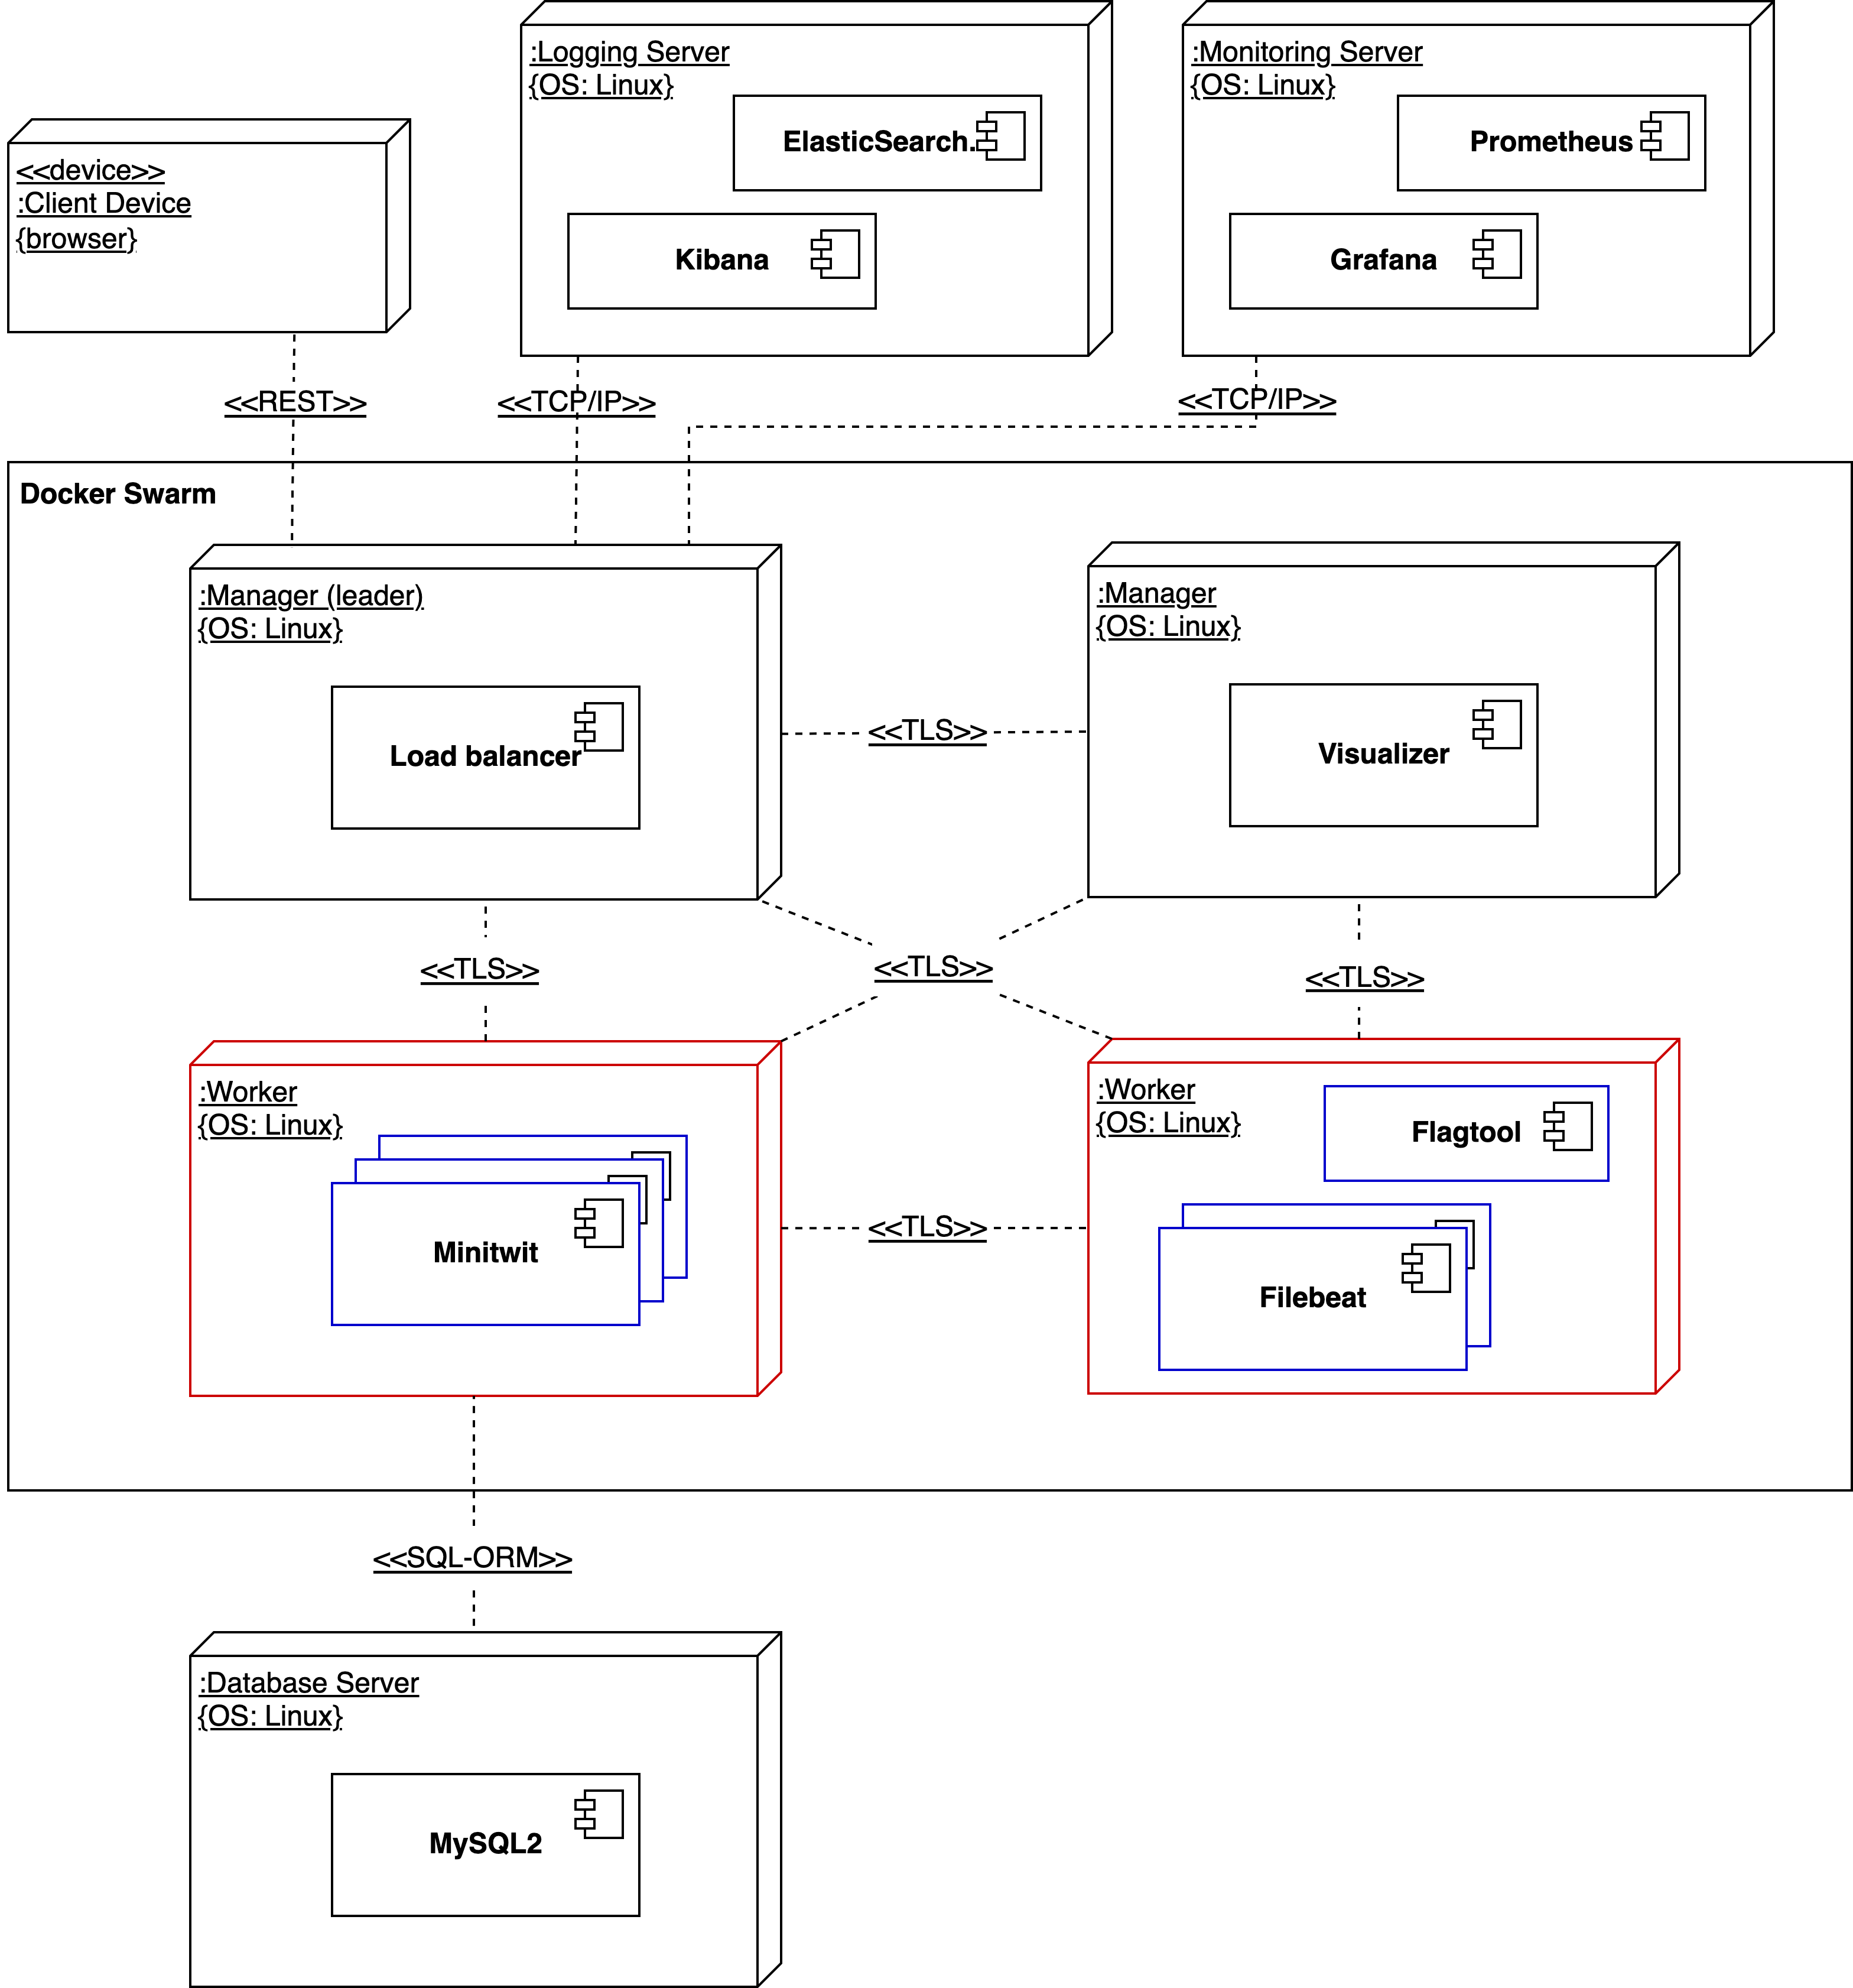
\includegraphics[width=\linewidth]{images/deployment-diagram.png}
    \caption{Deployment diagram of the Minitwit system}
    \label{fig:deployment-diagram}
\end{figure}


\subsection{Arguments for key technology/tool choices}

A list of all dependencies in the system can be found in Appendix \ref{app:dependencies}. \\

% OBS MSc students: Remember to log and provide good arguments for the choice of programming language and framework. Likely, a feature mapping/comparison or a mini-benchmark is a good choice. 

\textbf{Programming language and frameworks}\\
We chose JavaScript, as it is a popular and versatile language for web development that the team wanted to have more experience with. It also allows for a wide selection of front-end frameworks. We used the Pug library, allowing us to get started quickly and efficiently. While we initially considered transitioning to Vue.js or another modern framework for enhanced functionality, time constraints compelled us to prioritize the completion of mandatory assignments.\\ 

% OBS MSc students: Remember to log and provide good arguments for the choice of virtualization techniques and deployment targets 

\textbf{Virtualization technique and deployment targets}\\
We chose the containerization virtualization technique with cloud deployment. Containerization was chosen because of the apparent values it brings, such as being portable, ensuring that the application can run consistently in any environment, and being agile, since it is fast and easy to create, deploy, and destroy containers. We chose cloud deployment since none of the group members had the required setup for on-premise hosting and because of the convenience it brings, such as handling scaling and reduced infrastructure management. After shortly considering other opportunities, we selected DigitalOcean as our deployment platform, as suggested in the course.Among the most important benefits of the platform, we found an intuitive user experience and a 200 dollars credit included in accounts for academical purposes.
\\

% OBS MSc students: Remember to log and provide good arguments for the choice of ORM framework and chosen DBMS

\textbf{DBMS and ORM framework}\\
We opted to use MySQL as our chosen DBMS because it employs a relational data model, organizing data into tables and enforcing a fixed scheme. This structure aligns well with our application's needs, as it has a limited and well-defined set of data types. While PostgreSQL also supports this need and offers comparable features, the decision between MySQL and PostgreSQL was somewhat arbitrary due to their similar capabilities in this regard. As our ORM framework, we used Sequelize as it is widely used with Node.js applications and offers a comprehensive set of features for working with databases. Although it was compelling to try a self-hosted database to learn how to deal with infrastructure management, maintenance, backups, and disaster recovery planning, we decided to go with a hosted database option provided by DigitalOcean for its convenience and ease of use.

\subsection{Current state of the system}
%Describe the current state of your systems, for example using results of static analysis and quality assessments.

All the applications are fully functional. However, the system is currently shut down due to a lack of credits in DigitalOcean. We use SonarCloud as our quality management platform which runs automatic checks of our code after each pushed change. It detects potential vulnerabilities, bugs, code smells, and code duplication. Our codebase contains a significant number of code smells, primarily because our main focus was on addressing bugs and vulnerabilities rather than prioritizing their removal. Below, you can find a dashboard of the latest analysis in Figure \ref{fig:sonarCloud}. 

\begin{figure}[H]
    \centering
    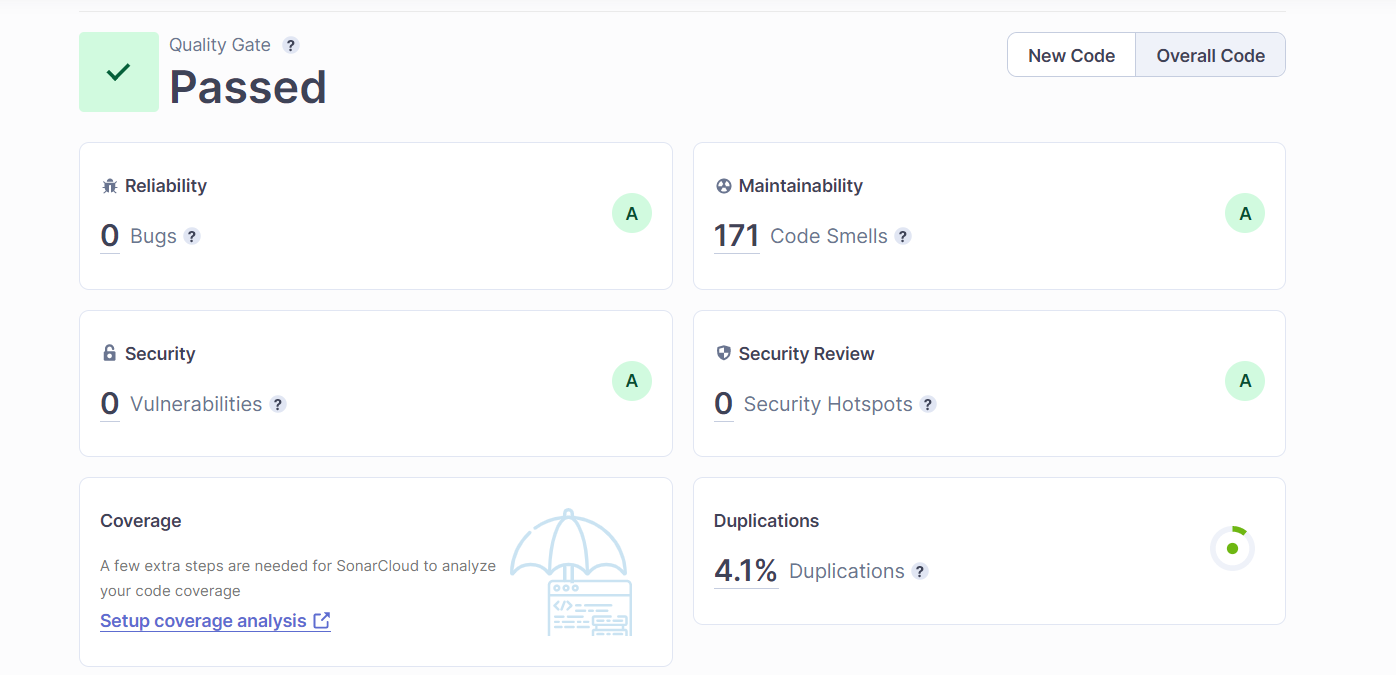
\includegraphics[width=\linewidth]{images/SonarCloud.png}
    \caption{SonarCloud analysis of our repository.}
    \label{fig:sonarCloud}
\end{figure}

\subsection{License}
We have chosen an MIT license since we using Node.js and npm packages are overwhelmingly using the MIT license or similar licenses \cite{choosealicense}. The license is added in our \texttt{root} folder. 

%Finally, describe briefly, if the license that you have chosen for your project is actually compatible with the licenses of all your direct dependencies.


% REMEMBER THE FOLLOWING:

%Double check that for all the weekly tasks (those listed in the schedule) you include the corresponding information.

%MSc students remember to argue for the choice of technologies and decisions for at least all cases for which we asked you to do so in the tasks at the end of each session.

